\documentclass[10pt]{article}
\usepackage{amsmath} 
\usepackage{fontspec}
\setmainfont{JetBrainsMono NFM}
\setmainfont[NFSSFamily=dayrom]{JetBrains Mono}
\usepackage[a4paper, margin=12mm]{geometry}
\usepackage{graphicx}
\graphicspath{ {./images/} }

\usepackage{amsmath}

\DeclareSymbolFont{digits}{TU}{dayrom}{m}{n}
\AtBeginDocument{
	\DeclareMathSymbol{0}{\mathalpha}{digits}{`0}
	\DeclareMathSymbol{1}{\mathalpha}{digits}{`1}
	\DeclareMathSymbol{2}{\mathalpha}{digits}{`2}
	\DeclareMathSymbol{3}{\mathalpha}{digits}{`3}
	\DeclareMathSymbol{4}{\mathalpha}{digits}{`4}
	\DeclareMathSymbol{5}{\mathalpha}{digits}{`5}
	\DeclareMathSymbol{6}{\mathalpha}{digits}{`6}
	\DeclareMathSymbol{7}{\mathalpha}{digits}{`7}
	\DeclareMathSymbol{8}{\mathalpha}{digits}{`8}
	\DeclareMathSymbol{9}{\mathalpha}{digits}{`9}
}

% Footer-Einstellungen
\usepackage{fancyhdr}
\usepackage{amsmath}
\usepackage{datetime}
\newdateformat{mydate}{\twodigit{\THEDAY}.\twodigit{\THEMONTH}.\THEYEAR}
\mydate
\pagestyle{fancy}
\fancyhf{} % Löscht alle Kopf- und Fusszeilen
\fancyfoot[C]{\thepage\ -\ \today\ \copyright\ Bastian\ Kind,\ James\ Binks,\ Mark\ Matkovic\ und\ David\ Hafner} % Setzt den Footer

\title{DFB Entdecker App}
\author{Bastian Kind, James Binks, Mark Matkovic und David Hafner}

\begin{document}
	\maketitle
	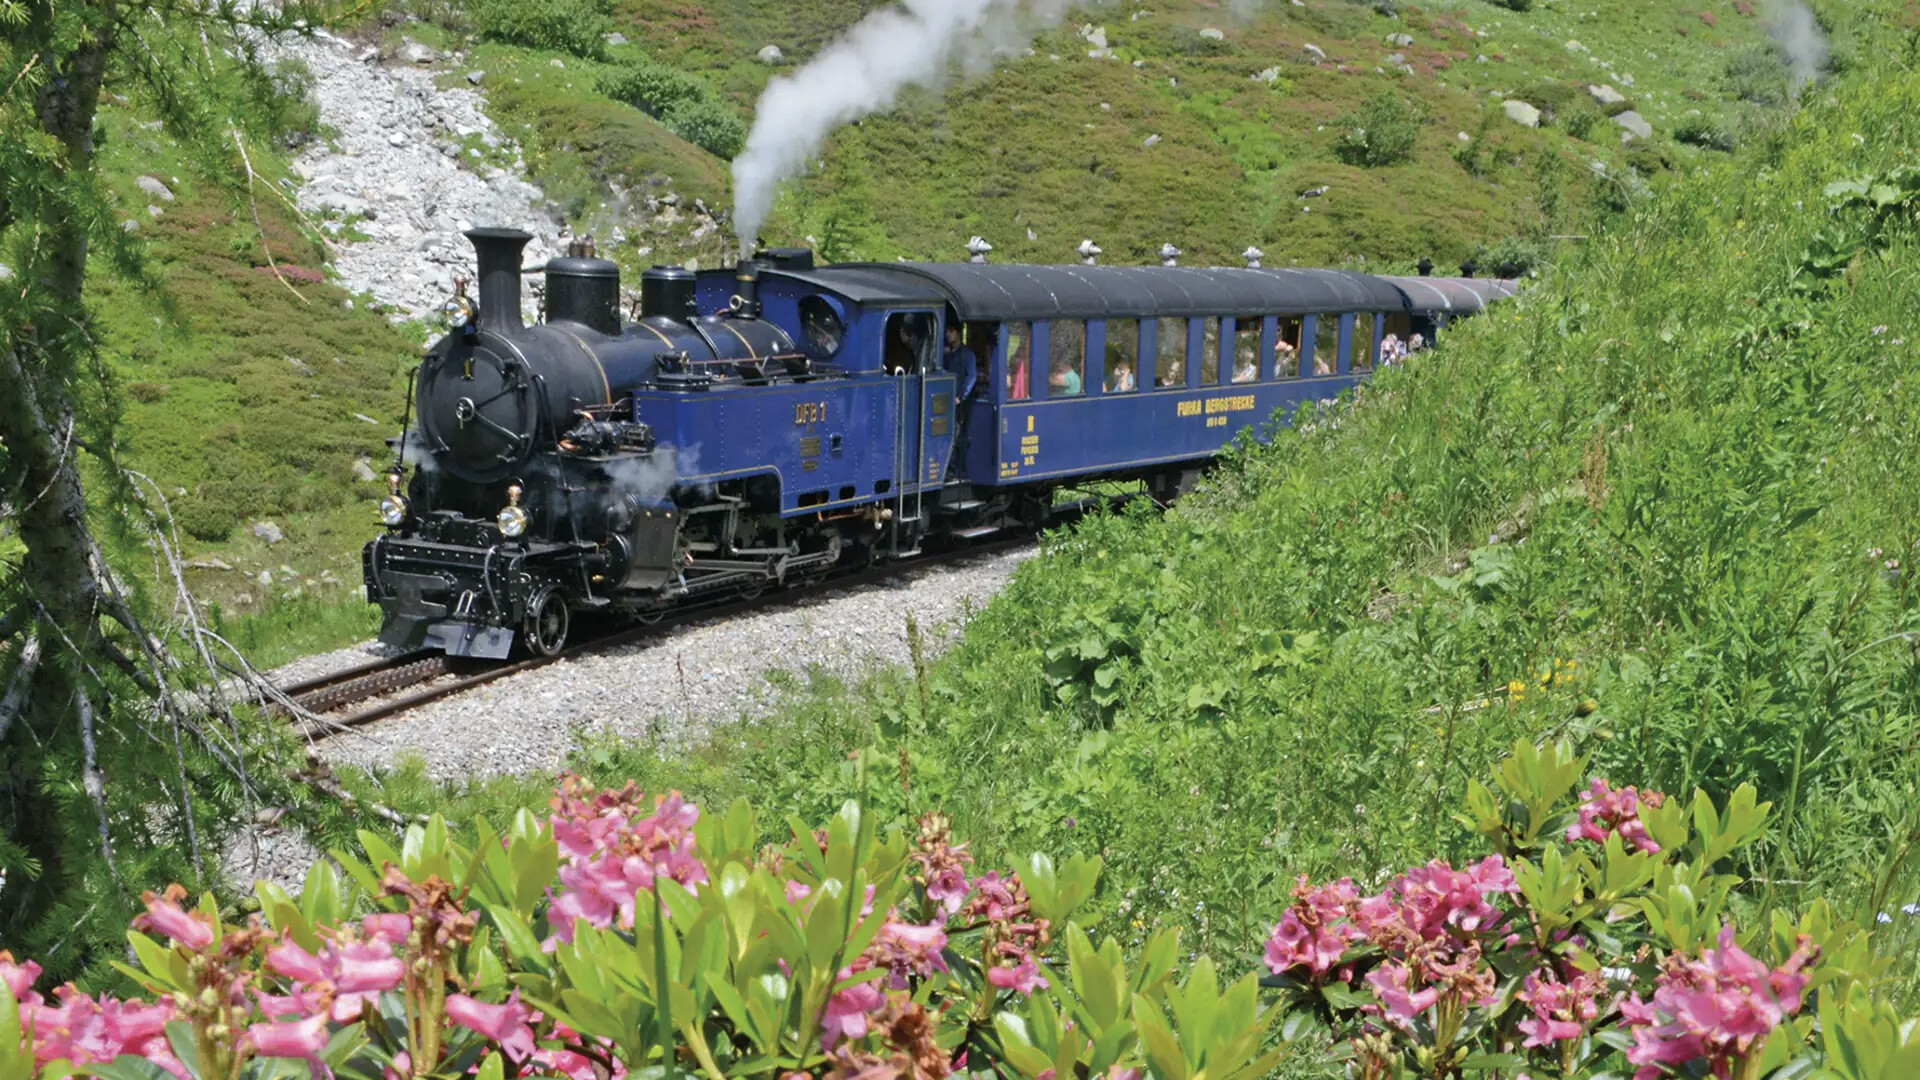
\includegraphics[width=17.5cm]{title}
	\pagebreak
	\tableofcontents
	\pagebreak
	\section{Band A}
	\subsection{Anforderungsanalyse}
	\subsubsection[Wer]{Wer benutzt die App?}
	\begin{itemize}
		\item Familien mit Kindern (z.\,B. als Freizeit-Ausflug)
		\item Rentner / ältere Menschen (Interesse an Geschichte und Eisenbahn)
		\item Erwachsene allgemein (z.\,B. Eisenbahnbegeisterte, Touristen)
		\item Schulklassen (für interaktive, spielerische Lernmöglichkeiten)
	\end{itemize}
	\subsubsection[Wo]{Wo wird die App verwendet?}
	\begin{itemize}
		\item Entlang der Furka-Bergstrecke, einer historischen Dampfbahnstrecke
		\item Draussen (z.B. auf Bahnhöfen, an Brücken, bei Aussichtspunkten)
		\item Oft ohne Mobilfunknetz -> App muss offlinefähig sein
		\item Unterwegs mit dem Zug oder zu Fuss an Haltepunkten
	\end{itemize}
	\subsubsection[Was]{Was muss die App können?}
	\begin{itemize}
		\item QR-Codes an Infopunkten scannen -> Inhalte anzeigen (Text, Bilder, Videos, Audio)
		\item Karte mit GPS nutzen -> aktuelle Position und nahegelegene Punkte anzeigen
		\item Quiz- oder Rätsel-Funktion -> spielerisches Lernen
		\item Tagebuch- oder Sammelfunktion («Meine liebsten Sehenswürdigkeiten»)
		\item Inhalte in mehreren Sprachen (D/E/F/I), evtl. auch einfache Sprache
		\item Inhalte offline verfügbar
		\item Datenschutzkonform -> keine Registrierung, keine Standortüberwachung
	\end{itemize}
	\subsubsection[Womit]{Technische Rahmenbedingungen}
	\begin{itemize}
		\item Smartphone oder Tablet, Android und iOS
		\item Ressourcenschonendes Design (damit es auch auf älteren Geräten läuft)
		\item App soll Inhalte aus CMS (z.\,B. Texte, Medien) beziehen
		\item Kein Internet nötig unterwegs (alle Inhalte offline verfügbar)
		\item Barrierefreiheit: Vorlesefunktion, grosse Schrift, starke Kontraste
	\end{itemize}
	\subsubsection[Verbesserungen]{Verbesserungen}
		\begin{itemize}
			\item Wir könnten die Benutzergruppen noch genauer unterteilen. Z.\,B. nach technischen Kentnissen, Alter oder ob die Nutzer einheimische oder Touristen sind.
			\item Wir könnten konkrete Anforderungen für barrierefreies Design formulieren. Z.\,B. Schriftgrössen, Bedienung mit Screenreader, Kontraste
			\item Wir könnten die Datenschutzanforderungen genauer definieren. Z.\,B. Wie werden die GPS Daten verarbeitet?
			%\item \textbf{Gamification weiterdenken:} Die Rätsel- und Sammelfunktionen könnten mit Badges, Levels oder Belohnungen erweitert werden, um die Motivation zu steigern.
		\end{itemize}
		\pagebreak
	\subsection{Vorgehensmodell}
		\subsubsection{Wahl des Modells}
		% Erklärung, welches Vorgehensmodell gewählt wurde (z. B. Design Thinking, User Centered Design) und warum
		Wir haben das Vorgehensmodell Design Thinking gewählt, da es gut zu unserem Projekt passt. Es ist benutzerorientiert und iterativ. Es gibt viel Nutzerfeedback und das Endprodukt ist das, was der Nutzer will.\\
		So können wir sicherstellen, dass wir uns nicht in Details verlieren, die dem Nutzer schlussendlich wenig nützen. Wir werden uns so besser auf die Wünsche und die Bedürfnisse des Nutzers konzentrieren können.
		\subsubsection{Phasen des Modells}
		% Beschreibung der einzelnen Phasen des gewählten Modells mit kurzer Erklärung (z. B. beim Design Thinking: Verstehen, Beobachten, Sichtweise definieren, Ideen finden, Prototyp bauen, Testen)
		Design Thinking hat zwei «Räume». Es gibt den Problemraum und den Lösungsraum. Im Problemraum schaut man die Probleme an.
		\begin{itemize}
			\item Verstehen
			\subitem Als erstes muss man das Umfeld und die Nutzer verstehen.
			\item Beobachten
			\subitem Dann schaut man, wie sich der Nutzer verhält.
			\subitem Was macht der Nutzer, was ist ihm am wichtigsten, womit verbringt er viel Zeit.
			\item Standpunkt definieren
			\subitem Die gewonnen Erkenntnisse muss man dann aufschreiben und nach Wichtigkeit filtern oder sortieren.
			\subitem Möglicherweise braucht man noch mehr Informationen und muss nochmals zu einem der beiden vorherigen Schritte zurückgehen.
		\end{itemize}
		Im Lösungsraum überlegt man sich dann Lösungen für die gefundenen Probleme.
		\begin{itemize}
			\item Ideen finden
			\subitem Im ersten Schritt im Lösungsraum überlegt man sich, wie man die Probleme lösen könnte
			\item Prototyp entwickeln
			\subitem Zu diesen Ideen entwickelt man dann einen Prototypen.
			\item Testen
			\subitem Diesen Prototypen testet man dann mit dem Nutzer
			\subitem Mit dem erhaltenen Feedback muss man dann evtl. Zu einem der vorherigen Schritte zurückkeren und Verbesserungen vornehmen.	
		\end{itemize}
		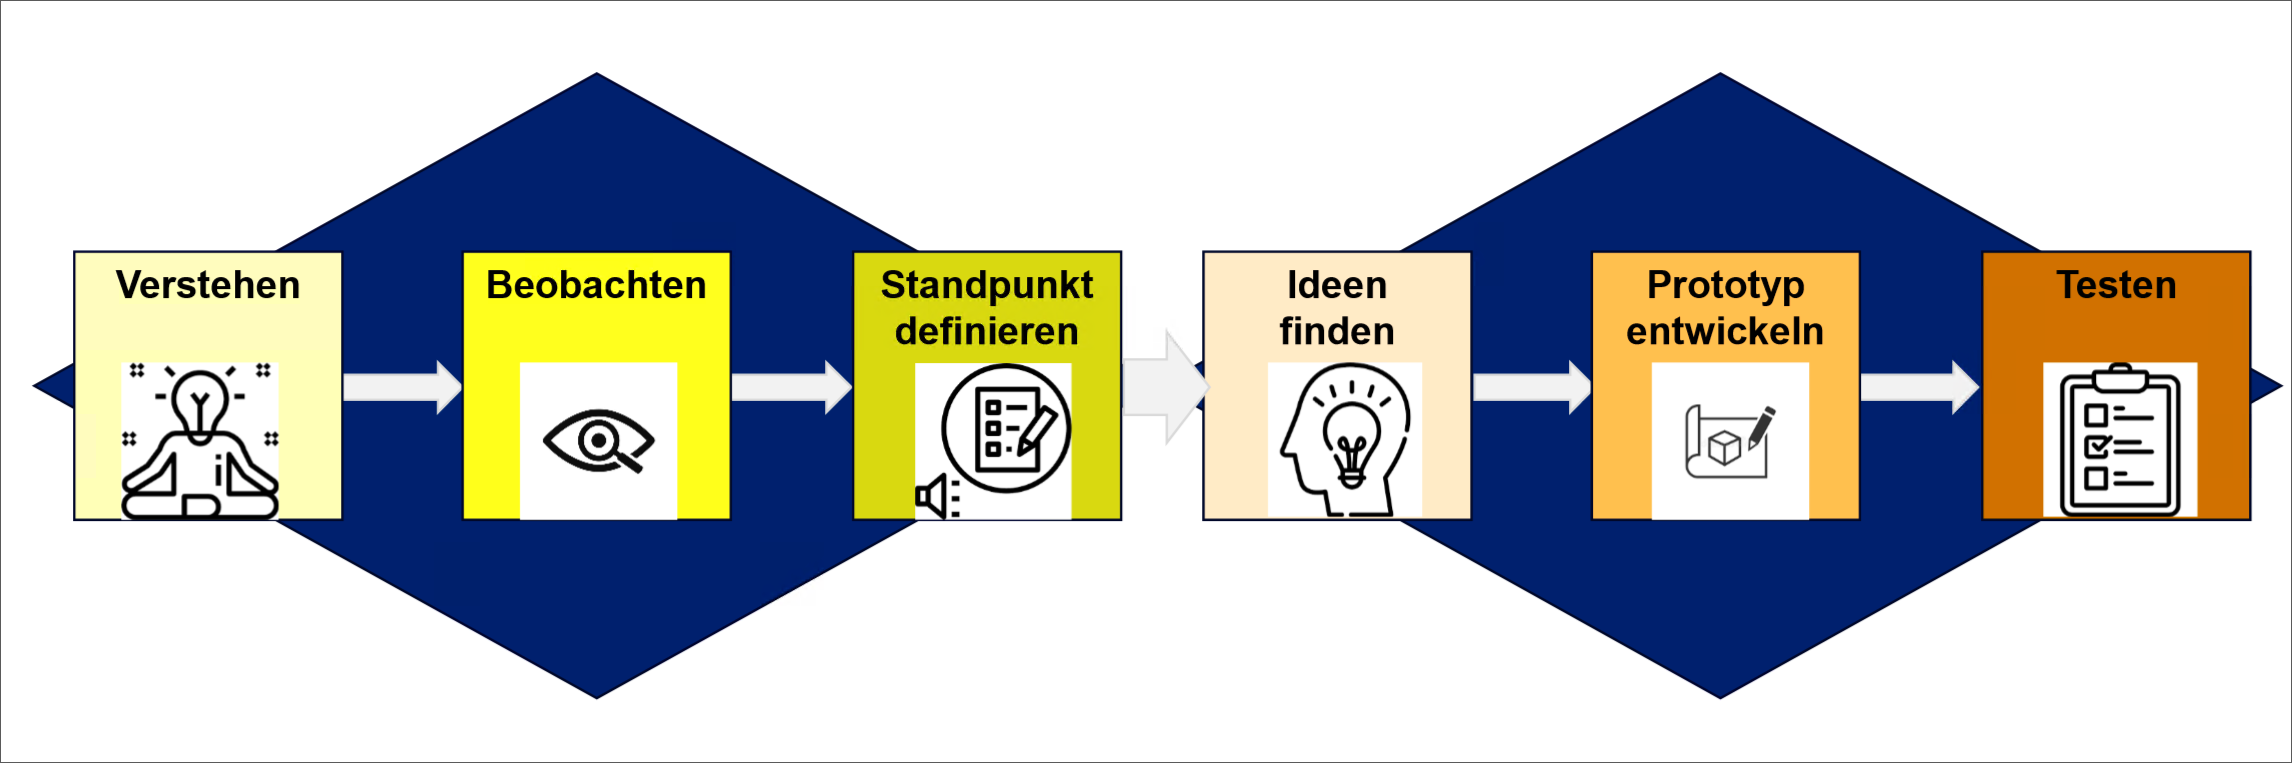
\includegraphics[width=18.6cm]{DesignThinking}
	\pagebreak
	\subsection{Nutzungskontext}
	
	\subsubsection{Methoden zur Kontextanalyse}
	
	\begin{itemize}
		\item Beobachtungen vor Ort entlang der Strecke
		\item Interviews mit Besuchern
		\item Analyse von Bewertungen der DFB
	\end{itemize}
	
	\subsubsection{Analyseergebnisse}
	\begin{itemize}
		\item Die Strecke liegt in einem abgelegenen Berggebiet – Mobilfunknetz ist nur teilweise verfügbar.
		\item Die Nutzung erfolgt draussen: an Bahnhöfen, Aussichtspunkten, Infotafeln oder im Zug.
		\item Nutzer sind häufig zu Fuss unterwegs und haben nur kurz Zeit für Interaktion.
		\item Zielgruppe ist sehr durchmischt: Kinder, Erwachsene, Senioren, Touristen, Schulklassen.
		\item Viele Nutzer wünschen sich eine spielerische, leicht verständliche und multilinguale Erfahrung.
	\end{itemize}
	
	\subsubsection{Schlussfolgerungen für die App}
	\begin{itemize}
		\item Die App muss vollständig offlinefähig sein.
		\item Eine einfache Bedienung ist nötig, besonders für Kinder und ältere Menschen.
		\item Barrierefreiheit ist wichtig: große Schrift, kontrastreiche Farben, Vorlesefunktion.
		\item Inhalte müssen mehrsprachig verfügbar sein (De/En/Fr/It), mit vereinfachtem Deutsch für Kinder.
		\item Die App sollte schnell Informationen liefern, da Nutzer meist unterwegs oder in Bewegung sind.
	\end{itemize}
	\pagebreak
	\subsection{Benutzereigenschaften}
	\pagebreak
	\subsection{Nutzungsanforderungen}
\end{document}